\documentclass[9pt]{article}
\usepackage[utf8]{inputenc}\usepackage[T1]{fontenc}\usepackage{lmodern}
\usepackage[letterpaper,top=.88cm,bottom=.88cm,left=1.02cm,right=1.02cm]{geometry}
\usepackage{graphicx,booktabs,amsmath,hyperref,array,tabularx,multicol,xcolor}
\definecolor{navy}{HTML}{102A43}\definecolor{blue}{HTML}{184E77}\definecolor{teal}{HTML}{2A9D8F}
\definecolor{pale}{HTML}{EDF5FB}\definecolor{red}{HTML}{C95745}\definecolor{ink}{HTML}{172033}\definecolor{muted}{HTML}{526B7A}
\hypersetup{colorlinks=true,urlcolor=blue,linkcolor=blue,pageanchor=false}
\setlength{\parindent}{0pt}\setlength{\parskip}{2.25pt}\setlength{\tabcolsep}{3.4pt}\renewcommand{\arraystretch}{1.07}
\newcolumntype{Y}{>{\raggedright\arraybackslash}X}
\newcommand{\pagetitle}[2]{{\color{navy}\LARGE\bfseries #1\par}\vspace{1pt}{\color{teal}\rule{\linewidth}{1.5pt}}\vspace{1pt}{\color{muted}\small #2\par}\vspace{4pt}}
\newcommand{\takeaway}[1]{\par\noindent\textcolor{navy}{\textbf{Conclusión.} #1}\par}
\newcommand{\warn}[1]{\par\noindent\textcolor{red}{#1}\par}
\newcommand{\subhead}[1]{\vspace{2pt}{\color{blue}\bfseries #1}\par}
\begin{document}

% 1 — PORTADA
\begin{titlepage}\pagecolor{navy}\color{white}
\vspace*{.25cm}{\small\bfseries DEEP LEARNING Y SISTEMAS INTELIGENTES\hfill PROYECTO 1 · V7\par}
\vspace{.35cm}{\color{teal}\rule{\linewidth}{2pt}}\vspace{.65cm}
{\Huge\bfseries Monitoreo transaccional\par}\vspace{.15cm}{\LARGE Selección train-only, orden y decisión económica\par}
\vspace{.55cm}{\large\bfseries Pregunta ejecutiva\par}\vspace{3pt}¿El orden o una arquitectura secuencial aportan señal incremental frente a un baseline tabular competitivo, y cuánto vale esa diferencia?
\vspace{.58cm}\begin{tabularx}{\linewidth}{@{}XXXX@{}}
\centering\textbf{590,540}\newline\scriptsize transacciones&\centering\textbf{3.50\%}\newline\scriptsize prevalencia&\centering\textbf{0.547}\newline\scriptsize AP interna A5&\centering\textbf{Q826,800}\newline\scriptsize costo interno A5
\end{tabularx}
\vspace{.58cm}{\color{teal}\Large\bfseries Decisión: conservar A5 como candidato exploratorio\par}\vspace{4pt}A5 combina el control V6 con modelos V7 y mejora AP, precisión, F1, costo y carga de alertas en promedio. No se declara superior de forma estable porque una de cuatro ventanas cae más de 0.005 AP; C no cumple su hipótesis y B no demuestra valor material del orden.
\vfill\begin{tabularx}{\linewidth}{@{}YY@{}}\textbf{Universidad del Valle de Guatemala}\newline Facultad de Ingeniería · Sección 30\newline Docente: Kevin Recinos · Semestre II 2026&\textbf{Equipo}\newline Wilson Alejandro Calderón Argueta · 22018\newline Pablo Daniel Barillas Moreno · 22193\end{tabularx}
\end{titlepage}\hypersetup{pageanchor=true}\setcounter{page}{1}\nopagecolor\color{ink}

% 2 — DATOS Y PROTOCOLO
\pagetitle{1 · Datos, EDA y protocolo temporal}{La mejora se evalúa con causalidad, transformaciones train-only y un benchmark explícitamente reutilizado.}
\takeaway{Se usaron las 590,540 transacciones y la unión completa de IEEE--CIS. IDs y tiempo crudo no son predictores; selección, correlación, imputación y PCA se ajustan solo con pasado.}
\begin{multicols}{2}
\subhead{Fuente y población} La fuente es \href{https://www.kaggle.com/competitions/ieee-fraud-detection/overview}{IEEE--CIS Fraud Detection}, publicada en Kaggle con datos anonimizados de Vesta Corporation. Las tablas se unen por \texttt{TransactionID} y se ordenan por \texttt{TransactionDT}. Hay 20,663 fraudes (3.50\%).

\subhead{Inventario} La unión produce 465 columnas después de ingeniería V7. Se retienen 460 variables candidatas; 34 representantes se eliminan únicamente por redundancia extrema ($|\rho_s|\ge0.995$). \texttt{TransactionID} se usa para alineación y \texttt{TransactionDT} para causalidad, nunca como magnitudes.

\subhead{Variables causales} Para una transacción $t$, toda estadística histórica cumple $x_t^{hist}=f(\{x_j:t_j<t\})$. Se añaden frecuencia previa de tarjeta/contexto, monto relativo, recencia, faltantes y resúmenes C/D/V/identidad. El evento actual no entra en sus propios agregados.

\subhead{Correlación y PCA} Spearman localiza redundancia dentro de train. PCA comprime solo \texttt{V1--V339}: 70 componentes explican 90\%, 105 explican 95\%; con 128 no se alcanza 99\%. Se valida la señal predictiva porque varianza explicada no equivale a fraude preservado.

\subhead{Identidad proxy} Se comparan tarjeta+dirección, tarjeta+dirección+correo y variantes con dispositivo/producto. Mayor cobertura no garantiza identidad correcta: las claves pueden mezclar clientes o fragmentar uno, limitando el significado de la secuencia.

\subhead{Walk-forward} Tres refits con preprocesamiento reaprendido logran AP 0.599, 0.466 y 0.603. La dispersión confirma deriva y justifica exigir estabilidad, no solo una media alta.
\end{multicols}
\subhead{Bloques cronológicos del protocolo}
\begin{tabularx}{\linewidth}{@{}p{2.15cm}p{1.8cm}Y Y@{}}\toprule
\textbf{Bloque}&\textbf{Fracción}&\textbf{Uso}&\textbf{Control}\\ \midrule
Train&70\% total&Preprocesamiento y modelos base&No observa validación\\
Early&0--35\% val&Early stopping&Anterior a selección\\
Meta fit&35--50\% val&Stacking A5 y C&Predicciones fuera de tiempo\\
Model select&50--60\% val&Elegir A y C&Dos subventanas\\
Calibración&60--70\% val&Probabilidades&Separada del umbral\\
Umbral&70--80\% val&$4200FN+180FP$, recall $\ge.75$&Regla congelada\\
Evaluación&80--100\% val&Gates y veredicto&No reajusta modelos\\
Benchmark&15\% total&Referencia histórica&No es test ciego\\ \bottomrule
\end{tabularx}
\vfill\warn{El benchmark fue observado en V1--V6; una afirmación confirmatoria requiere una cohorte futura etiquetada.}
\clearpage

% 3 — A Y RESULTADOS
\pagetitle{2 · Modelos A y reducción dimensional}{La mejor mejora no es un modelo aislado: es un stacking que conserva el baseline fuerte y añade señales complementarias.}
\begin{tabularx}{\linewidth}{@{}p{1.2cm}p{3.4cm}Y r@{}}\toprule
\textbf{Modelo}&\textbf{Diseño}&\textbf{Propósito}&\textbf{AP select}\\ \midrule
A0&Regresión logística · 100 variables&Control lineal&0.286\\
A1&LightGBM · variables ampliadas&Sin reducción&0.569\\
A2&LightGBM · $|\rho_s|<0.995$&Compactar redundancia&0.576\\
A3&LightGBM · PCA V (128)&Comprimir bloque anónimo&0.513\\
A4&CatBoost · categóricas nativas&Interacciones categóricas&0.428\\
\textbf{A5}&\textbf{Stacking A0--A4 + control V6}&\textbf{Complementariedad fuera de tiempo}&\textbf{0.628}\\ \bottomrule
\end{tabularx}
\begin{minipage}[c]{.51\linewidth}\centering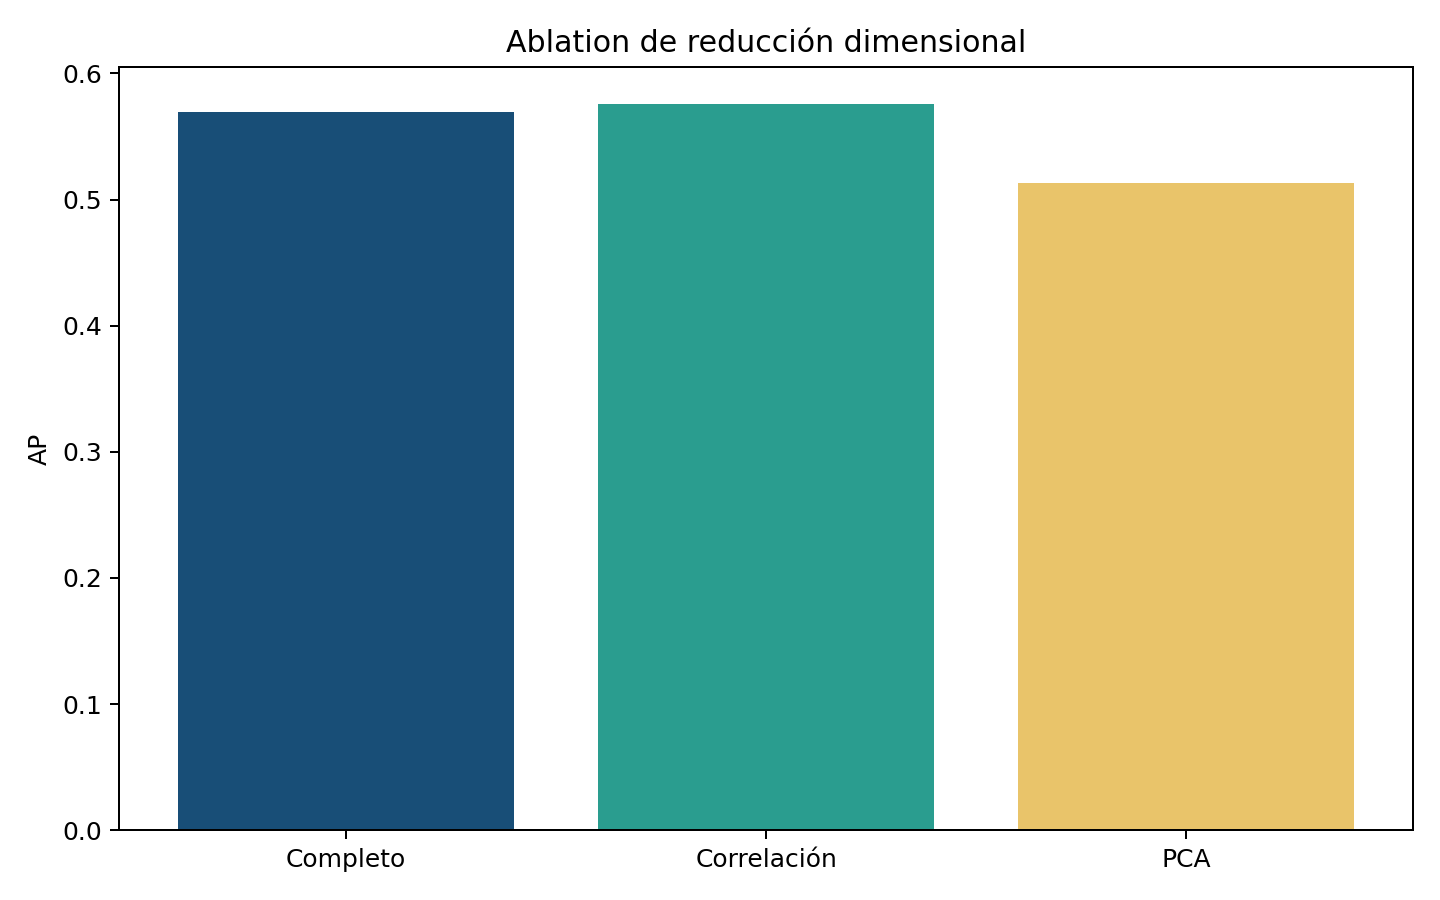
\includegraphics[width=\linewidth]{../../../evidencia/figuras/v7/04_correlacion_pca_v7.png}\end{minipage}\hfill
\begin{minipage}[c]{.46\linewidth}\small
\textbf{Resultado de la ablation.} A2 supera ligeramente A1 en selección, pero ambos caen en evaluación. PCA pierde señal y CatBoost tampoco gana individualmente. El resultado evita dos conclusiones fáciles pero falsas: ``menos variables siempre generaliza mejor'' y ``categóricas nativas garantizan superioridad''.

\textbf{Por qué A5 sí ayuda.} El metamodelo logístico usa logits de A0--A4 y del control V6, todos generados en períodos posteriores al entrenamiento base. Se ajusta en \texttt{meta\_fit}; su ventaja se comprueba después. Incluir V6 corrige una omisión inicial y evita descartar el baseline más fuerte.
\end{minipage}
\subhead{Evaluación temporal interna común}
\begin{center}\scriptsize\begin{tabular}{lrrrrrrrr}\toprule Modelo&AP&ROC&Prec.&Recall&F1&Costo&Alertas/100k&P@1\%\\ \midrule
\textbf{A}&\textbf{0.547}&\textbf{0.913}&\textbf{0.198}&0.772&\textbf{0.315}&\textbf{Q826,800}&\textbf{11,966}&\textbf{0.887}\\
B&0.392&0.853&0.112&0.708&0.194&Q1,215,900&19,360&0.723\\
C&0.543&0.913&0.194&\textbf{0.781}&0.311&Q818,040&12,378&0.881\\
D&0.217&0.758&0.054&0.743&0.101&Q1,854,120&41,982&0.497\\ \bottomrule
\end{tabular}\end{center}
\takeaway{A5 mejora AP +0.0111 y reduce costo 8.68\% frente a V6 en promedio interno, con precisión 19.8\% y recall 77.2\%. El gate de estabilidad sigue siendo negativo por una ventana.}
\clearpage

% 4 — ORDEN
\pagetitle{3 · Valor del orden y modelo B}{Una arquitectura secuencial no demuestra orden por diseño: la predicción debe degradarse cuando sus antecedentes se barajan.}
\begin{minipage}[c]{.60\linewidth}\centering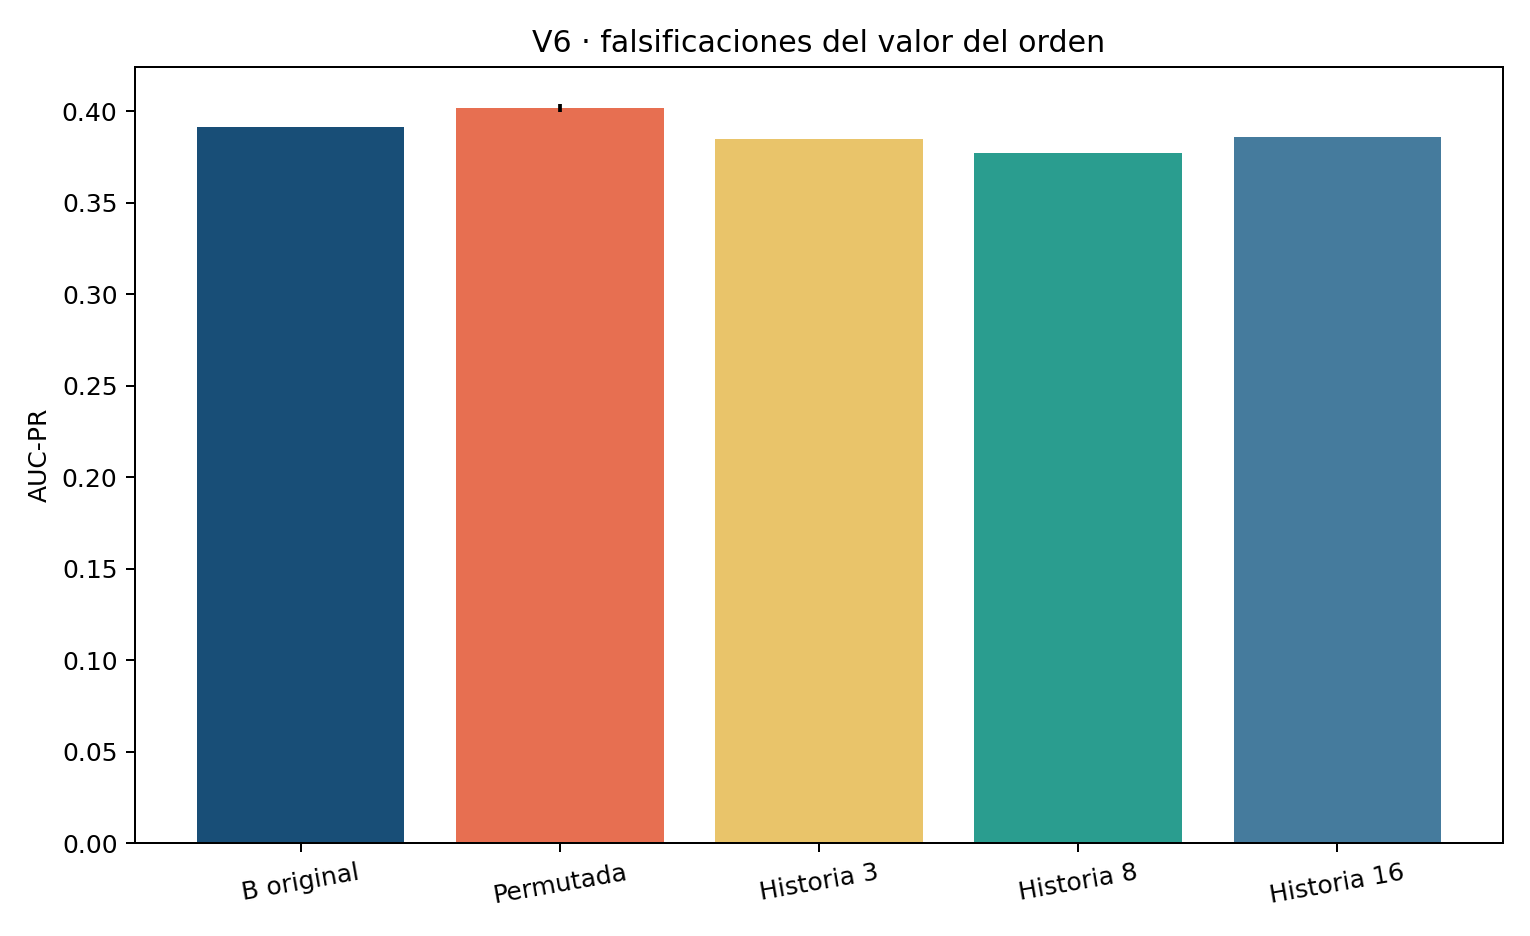
\includegraphics[width=\linewidth]{../../../evidencia/figuras/v6/03_falsificaciones_orden_v6.png}\end{minipage}\hfill
\begin{minipage}[c]{.37\linewidth}\small\begin{tabularx}{\linewidth}{@{}Y r@{}}\toprule Condición&AP\\ \midrule
B original · 32&0.3915\\ Permutada · 5 semillas&0.4016$\pm$0.0023\\ Historia 3&0.3847\\ Historia 8&0.3774\\ Historia 16&0.3860\\ Historia 32&0.3915\\ \bottomrule\end{tabularx}\end{minipage}
\subhead{Falsificación 1 · permutación controlada} Se mantiene la transacción objetivo al final y se barajan solo antecedentes. La diferencia original--permutada es $-0.0101$ AP: destruir el orden mejora el ranking promedio, opuesto a la caída positiva mínima de 0.01 requerida.

\subhead{Falsificación 2 · longitud} Los recortes 3/8/16 y la historia completa 32 se evalúan sin reentrenar, por lo que aíslan sensibilidad inferencial, no capacidad óptima de cada longitud. No aparece un crecimiento monotónico; ampliar la ventana no aporta evidencia útil.

\subhead{Qué sí y qué no significa} B logra AP 0.392, muy por encima de prevalencia: contiene señal. Sin embargo, queda por debajo de A y puede apoyarse en el evento actual o la composición del conjunto histórico, no en su orden. La identidad proxy ruidosa explica por qué más antecedentes pueden añadir mezcla en vez de memoria.

\begin{tabularx}{\linewidth}{@{}p{3.1cm}Y Y@{}}\toprule Pregunta&Resultado&Conclusión permitida\\ \midrule
¿B predice mejor que azar?&Sí; AP $\gg$ 0.035&B aprende señal\\
¿B supera A5?&No; pierde 0.156 AP&A es más competitivo\\
¿B usa favorablemente el orden?&No; permutar eleva AP&No atribuir valor material\\
¿Más historia ayuda?&Sin patrón monotónico&No aumentar longitud sin mejor identidad\\ \bottomrule
\end{tabularx}
\vfill\takeaway{Con la identidad, representación y TCN disponibles, el orden no aporta señal incremental demostrable. Una red más grande no corrige este resultado experimental.}
\clearpage

% 5 — C Y D
\pagetitle{4 · Apuesta C y encoder--decoder D}{La complementariedad y la anomalía se aceptan solo si mejoran ranking, costo y estabilidad bajo reglas previas.}
\begin{multicols}{2}
\subhead{Hipótesis C} C sería útil con $\Delta AP\ge0.01$, reducción de costo $\ge5\%$, recall $\ge.75$, alertas $\le+10\%$ y mejora en tres de cuatro ventanas. Se comparan C1=A+B, C2=A+B+D y C3 condicionada por calidad, historia, monto y faltantes. C1 gana selección con AP 0.638.

\subhead{Veredicto C} Frente a A, C1 cambia AP en $-0.0047$, reduce costo 1.06\%, aumenta alertas 3.44\% y no mejora ninguna ventana. Aunque su recall es algo mayor, falla AP, ahorro y estabilidad: \textbf{C no se promueve}.

\subhead{Diseño D} El autoencoder aprende solo transacciones legítimas y minimiza $\mathcal L_{AE}=p^{-1}\sum_j(x_j-\hat x_j)^2$. Su error se transforma en percentil respecto de errores legítimos de referencia y luego se calibra.

\subhead{Qué obtuvo D} AP 0.217, precisión 0.054 y 41,982 alertas/100k muestran que anomalía no equivale a fraude. Operaciones legítimas raras, deriva y faltantes también reconstruyen mal. D queda como control y entrada opcional de C, no como candidato.

\subhead{Calibración} Cada score se recalibra en un bloque separado. El Brier de A es 0.0193 interno; calibrar no cambia AP porque preserva el orden, pero permite interpretar el umbral y comparar costo.

\subhead{Lectura metodológica} El resultado negativo de C es evidencia útil: B/D no añaden señal suficientemente complementaria. Reajustar C con el benchmark violaría el protocolo. La siguiente prueba debe usar predicciones out-of-fold más diversas y una cohorte nueva.
\end{multicols}
\begin{center}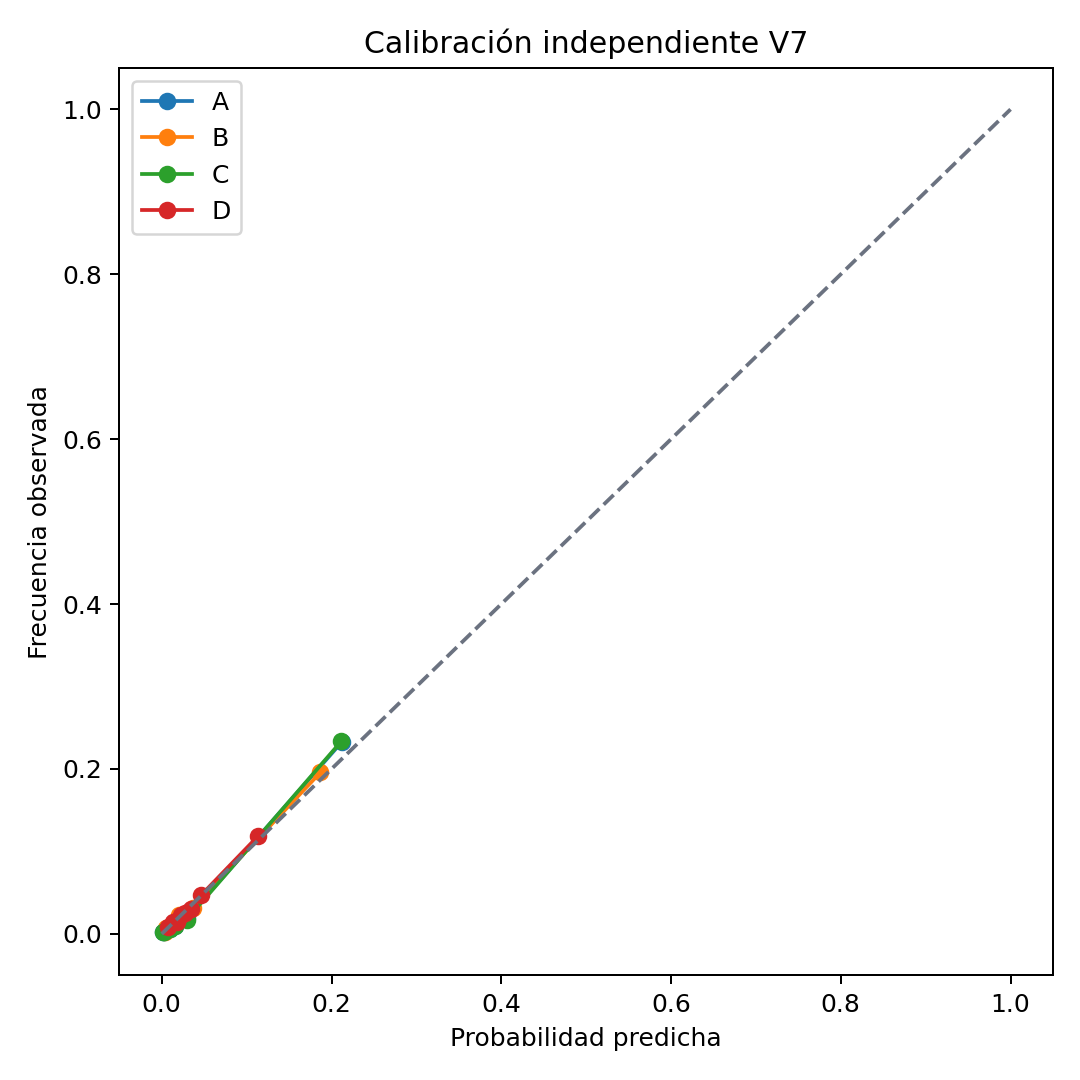
\includegraphics[width=.59\linewidth]{../../../evidencia/figuras/v7/06_calibracion_v7.png}\end{center}
\vfill\warn{No se promueve C por su buen aspecto descriptivo en el benchmark; el veredicto se fijó antes, en evaluación interna.}
\clearpage

% 6 — ECONOMÍA
\pagetitle{5 · Economía, estabilidad y benchmark histórico}{FN cuesta 23.3 veces FP; por eso el umbral acepta alertas, pero V7 reduce sustancialmente esa carga.}
\begin{minipage}[c]{.50\linewidth}\centering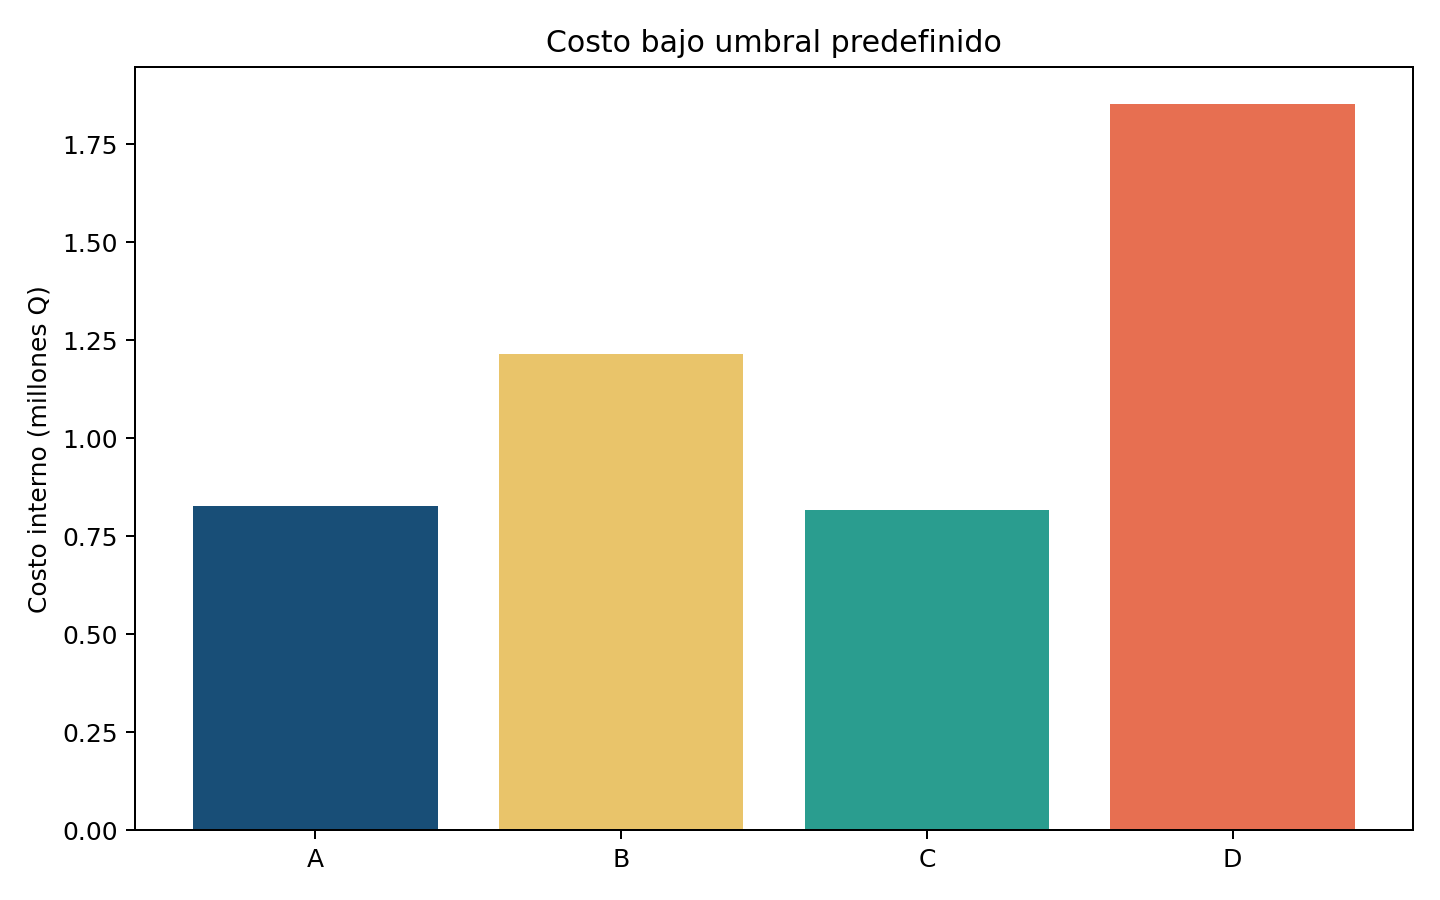
\includegraphics[width=\linewidth]{../../../evidencia/figuras/v7/05_costos_v7.png}\end{minipage}\hfill
\begin{minipage}[c]{.47\linewidth}\small
\[C(\tau)=Q4{,}200\,FN(\tau)+Q180\,FP(\tau).\]
A usa $\tau=0.05000$. Detecta 420 fraudes, omite 124 y produce 1,700 falsas alarmas: Q826,800. Frente a V6 conserva recall superior a 0.75, reduce alertas 28.6\% y costo 8.68\%.

\textbf{Gate.} AP global mejora 0.0111 y tres de cuatro ventanas son positivas (+0.0244, +0.0070, $-0.0135$, +0.0227). La tercera cae más de 0.005; el resultado es prometedor, no estable.
\end{minipage}
\subhead{Benchmark temporal histórico reutilizado}
\begin{center}\scriptsize\begin{tabular}{lrrrrrrr}\toprule Modelo&AP&ROC&Prec.&Recall&F1&Costo&Alertas/100k\\ \midrule
\textbf{A}&0.566&0.918&\textbf{0.210}&0.780&\textbf{0.331}&Q4,477,680&\textbf{12,938}\\
B&0.465&0.877&0.125&0.784&0.215&Q5,854,920&21,878\\
C&\textbf{0.571}&\textbf{0.919}&0.205&0.789&0.325&\textbf{Q4,436,880}&13,397\\
D&0.229&0.769&0.056&\textbf{0.824}&0.105&Q9,969,180&51,061\\ \bottomrule
\end{tabular}\end{center}
\subhead{Interpretación} AP 0.566 significa un ranking muy superior a la prevalencia 0.035, no que 56.6\% de alertas sea fraude. La precisión puntual es 21.0\%: aproximadamente una de cinco alertas es positiva. Recall 78.0\% implica recuperar casi ocho de diez fraudes. ROC 0.918 mide separación global, pero no cuantifica carga operativa; por eso se acompaña de AP, precisión, alertas y costo.

\subhead{Comparación honesta} En el benchmark, A5 eleva AP 0.0064, precisión 5.2 puntos, F1 0.067 y reduce costo Q406,020 frente al control V6, con recall 2.8 puntos menor. C luce mejor descriptivamente, pero su hipótesis interna fue rechazada. El benchmark no puede revocar esa decisión.
\vfill\takeaway{V7 mejora la utilidad operativa y reduce falsas alarmas; la evidencia de estabilidad todavía es insuficiente para declarar reemplazo confirmatorio.}
\clearpage

% 7 — CIERRE
\pagetitle{6 · Matriz de evidencias y decisión final}{Cada afirmación queda vinculada con una prueba, una conclusión permitida y una limitación explícita.}
\scriptsize\begin{tabularx}{\linewidth}{@{}p{2.2cm}p{2.6cm}Y Y@{}}\toprule Evidencia&Artefacto&Conclusión&Limitación\\ \midrule
Integridad&EDA, protocolo, contrato&590,540 filas; transformaciones train-only&Identidad aproximada\\
A competitivo&Selección A0--A5&A5 gana selección y mejora promedio interno&Una ventana se degrada\\
A/B común&Figura 1, scores&A supera B en AP, precisión, F1 y costo&B congelado desde V6\\
Valor del orden&5 permutaciones; 3/8/16/32&Permutar no perjudica; sin valor material&Recortes sin reentrenar\\
Apuesta C&Hipótesis y tres controles&C1 no alcanza AP ni ahorro predefinidos&Familia de fusión limitada\\
Encoder--decoder&Checkpoint/score D&Rareza tiene recall, no pureza&Normalidad multimodal\\
Economía&Curvas, figura 5&A5 reduce costo/alertas frente a V6&Costos académicos\\
Estabilidad&3 walk-forward + 4 ventanas&Deriva material; promoción no confirmada&Sin cohorte futura\\ \bottomrule
\end{tabularx}
\subhead{Decisión concluyente} Conservar \textbf{A5} como candidato exploratorio V7 porque presenta el mejor equilibrio interno entre AP, precisión, F1, costo y alertas. No afirmar que V7 reemplaza definitivamente V6: incumple el gate de estabilidad. No promover B porque no supera A ni demuestra uso favorable del orden; no promover C porque falla su hipótesis; no promover D porque su baja precisión multiplica falsas alarmas.

\subhead{Qué cambiaría la decisión} (1) repetir la ganancia en una cohorte futura congelada; (2) evitar una caída mayor de 0.005 AP en todas las ventanas; (3) obtener identidad bancaria fiable y caída $\ge0.01$ al permutar; (4) que C logre simultáneamente $+0.01$ AP, $-5\%$ costo y recall $\ge.75$; (5) sustituir costos académicos por capacidad y costos reales.

\subhead{Límites y candidato al proyecto final} Datos anonimizados; identidad proxy; benchmark reutilizado; B/D congelados; costo académico; sin auditoría productiva de privacidad, equidad, explicabilidad, seguridad, latencia ni deriva futura. Entrada: transacción y agregados causales definidos en el contrato. Salida: \texttt{risk\_score} calibrado y umbral 0.05000. Faltantes y categorías nuevas siguen el preprocesamiento train-only.

\subhead{Uso de inteligencia artificial} Se utilizó asistencia de IA para estructurar código, revisar consistencia, automatizar entregables y redactar documentación. Los autores ejecutaron el pipeline, verificaron IDs, particiones, métricas, gates, artefactos y conclusiones, y deben poder defender las decisiones.

\subhead{Referencias APA 7}
IEEE Computational Intelligence Society. (2019). \textit{IEEE--CIS Fraud Detection} [Data set]. Kaggle. \url{https://www.kaggle.com/competitions/ieee-fraud-detection/overview}\\
Ke, G., et al. (2017). LightGBM: A highly efficient gradient boosting decision tree. \textit{Advances in Neural Information Processing Systems, 30}.\\
Prokhorenkova, L., et al. (2018). CatBoost: Unbiased boosting with categorical features. \textit{NeurIPS, 31}.\\
Saito, T., \& Rehmsmeier, M. (2015). The precision--recall plot is more informative than ROC for imbalanced data. \textit{PLOS ONE, 10}(3), e0118432.\\
Zhou, C., \& Paffenroth, R. C. (2017). Anomaly detection with robust deep autoencoders. \textit{Proceedings of KDD}, 665--674.
\vfill\takeaway{V7 mejora el promedio y la operación, pero el resultado científico principal es más preciso: hay señal tabular complementaria, no evidencia de orden y todavía no hay superioridad temporal estable.}
\end{document}
